%%%%%%%%%%%%%%%%%%%%%%%%%%% COORDINATESYSTEMS
% COORDSYS (ORIGOCOORDINATENAME, WIDTH, HEIGHT)
% Draws a Coordinatesystem around ORIGOCOORDINATENAME with a width of WIDTH and a height of HEIGHT, 
% names the beginning and end of axes, southwest corner, northwest corner, 
\newcommand{\CoordSys}[3]{%
\coordinate (XY#1) at ([xshift=#2 cm, yshift=#3 cm]#1);%
\coordinate (-XY#1) at ([xshift=-#2 cm, yshift=-#3 cm]#1);%
\coordinate (-X#1) at ([xshift=-#2 cm]#1);%
\coordinate (X#1) at ([xshift=#2 cm]#1);%
\coordinate (Y#1) at ([yshift=#3 cm]#1);%
\coordinate (-Y#1) at ([yshift=-#3 cm]#1);%
\draw [help lines, step=.5cm] (-XY#1) grid (XY#1);%
\draw[->] (-X#1)--(X#1);%
\draw[->] (-Y#1)--(Y#1);%
}

%Lorentz(OriginalOriginCoord, ResultingOriginCoord, SpeedNum, PointCoord, Label)
% 
\newcommand{\Lorentz}[5]{%
\path (#1); \pgfgetlastxy{\XCoord}{\YCoord}; % Extracting coordinates of the Origin
\pgfmathsetmacro{\XOrigin}{\XCoord} % Saving X coordinate
\pgfmathsetmacro{\YOrigin}{\YCoord} % Saving Y coordinate
\path (#4); \pgfgetlastxy{\XCoord}{\YCoord}; % Extracting coordinates of the Point
\pgfmathsetmacro{\XEvent}{\XCoord} % Saving X coordinate
\pgfmathsetmacro{\YEvent}{\YCoord} % Saving Y coordinate
\pgfmathsetmacro{\XEventWRTOrigin}{\XEvent-\XOrigin} % Relativizing to the origin
\pgfmathsetmacro{\YEventWRTOrigin}{\YEvent-\YOrigin} % Relativizing to the origin
\pgfmathparse{XLorentz(#3,\XEventWRTOrigin,\YEventWRTOrigin)} % transforming x
\pgfmathsetmacro{\XEventTr}{\pgfmathresult} % save the result of x
\pgfmathparse{YLorentz(#3,\XEventWRTOrigin,\YEventWRTOrigin)} % transforming y
\pgfmathsetmacro{\YEventTr}{\pgfmathresult} % save the result of y
\node[world](#5) at (
[xshift=\XEventTr pt,
 yshift=\YEventTr pt] #2){};
}

\usetikzlibrary{calc}
\newdimen\XCoord
\newdimen\YCoord

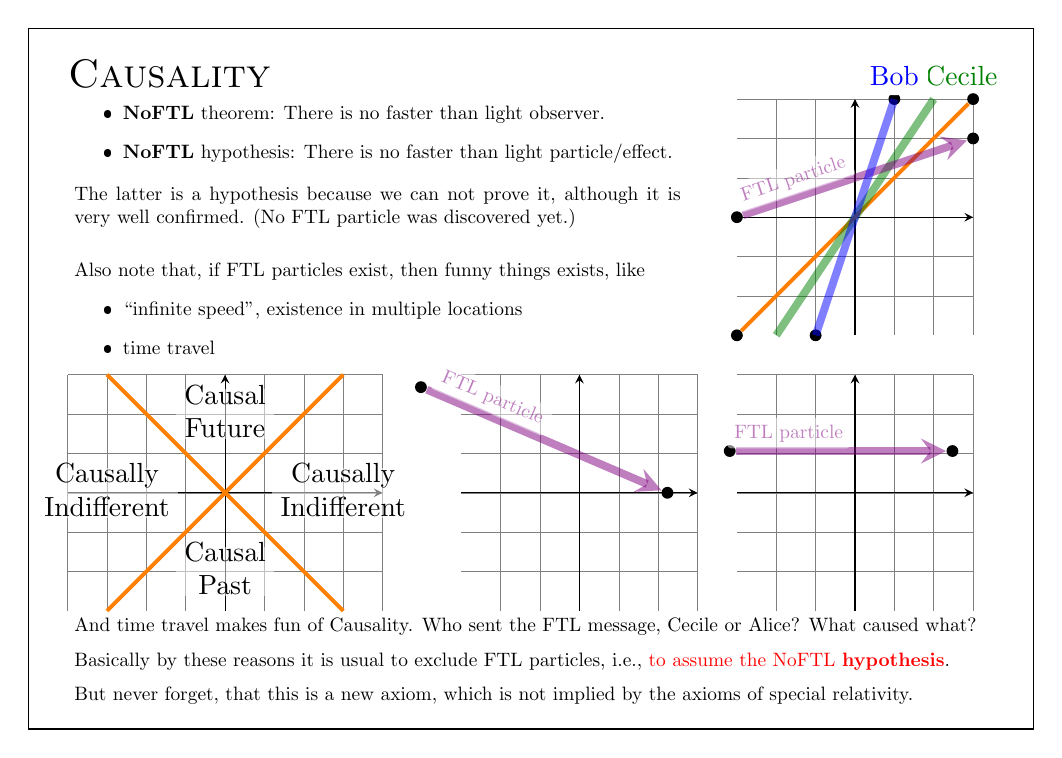
\begin{tikzpicture}[>=stealth, scale=1,
world/.style={inner sep=0, minimum size=.15cm, fill=black, circle},
worldline/.style={line width=1mm, rounded corners=1pt, opacity=.5},
axis/.style={->},
light/.style={orange, line width=.5mm},
]
\pgfmathdeclarefunction{XLorentz}{3}{\pgfmathparse{(#2 - #1*#3)/(sqrt(1-#1^2))}} % speed, spacecoord, timecoord
\pgfmathdeclarefunction{YLorentz}{3}{\pgfmathparse{(#3 - #1*#2)/(sqrt(1-#1^2))}} % speed, spacecoord, timecoord

%%%%%%%%%%%%%%%%%%%%%%%% DIA KEZDETE %%%%%%%%%%%%%%%%%%%%%%%%%%%

\node[anchor=north west, inner sep=0] at (0.5,8.5) {\textsc{\Large Causality}}; %%%%%%% TITLE
\draw%[white]  %%%%%%%%%%%% SIZE OF THE SLIDE
      (0,0) rectangle (12.77,8.9);
%%%%%%%%% TEXT %%%%%%%%%%%%%
\node[anchor=north west, scale=.7] at (0.5,8) {\begin{minipage}{11cm}
\begin{itemize}
\item \textbf{NoFTL} theorem: There is no faster than light observer.
\item \textbf{NoFTL} hypothesis: There is no faster than light particle/effect.
\end{itemize}
The latter is a hypothesis because we can not prove it, although it is very well confirmed. (No FTL particle was discovered yet.)
\end{minipage}
};
%%%%%%%%%%%%%%%%%%%%%%%% KOORDINÁTARENDSZEREK %%%%%%%%%%%%%%%%%%%%%%%%%%%
\coordinate(O1) at (10.5,6.5) {} {};
  \CoordSys{O1}{1.5}{1.5}
\coordinate(O2) at (10.5,3) {} {} {};
  \CoordSys{O2}{1.5}{1.5}
\coordinate(O3) at (7,3) {} {} {} {};
  \CoordSys{O3}{1.5}{1.5}
\coordinate(O4) at (2.5,3) {} {} {} {} {} {};
  \CoordSys{O4}{2}{1.5}

%%%%%%%%%%
%% SETTINGS %%
%%%%%%%%%%

\coordinate (SignalStart) at (9,5) {} {} {} {} {};
\coordinate (SignalBounced) at (12,8) {} {} {} {};
\coordinate (AliceStart) at (10.5,5) {} {} {} {};
\coordinate (AliceEnd) at (10.5,8) {} {} {} {};
\coordinate (BobStart) at (10,5) {} {} {} {} {} {} {}; % Fontos hogy átmenjen az Origón, különben rossz a lorentz transzformáció!!
\coordinate (BobEnd) at (11,8) {} {} {} {} {} {} {};
\coordinate (CecileStart) at (9.5,5) {} {} {} {} {} {} {} {}; % Fontos hogy átmenjen az Origón, különben rossz a lorentz transzformáció!!
\coordinate (CecileEnd) at (11.5,8) {} {} {} {} {} {} {} {};
\coordinate(FTLStart) at (9,6.5) {} {};
\coordinate(FTLEnd) at (12,7.5) {} {};

%%%%%%%%%%% Ezt lehetne macronak, speedszámítócuccnak
\path (BobStart); \pgfgetlastxy{\XCoord}{\YCoord}; % Extracting coordinates of the Origin
\pgfmathsetmacro{\XFirst}{\XCoord} % Saving X coordinate
\pgfmathsetmacro{\YFirst}{\YCoord} % Saving Y coordinate
\path (BobEnd); \pgfgetlastxy{\XCoord}{\YCoord}; % Extracting coordinates of the Point
\pgfmathsetmacro{\XSecond}{\XCoord} % Saving X coordinate
\pgfmathsetmacro{\YSecond}{\YCoord} % Saving Y coordinate
\pgfmathsetmacro{\SpeedBob}{(\XFirst-\XSecond)/(\YFirst-\YSecond)} % Relativizing to the origin
%%%%%%%%%%%%%%%%%%%%%%%%%%%%%%%%%%%
%%%%%%%%%%% Ezt lehetne macronak, speedszámítócuccnak
\path (CecileStart); \pgfgetlastxy{\XCoord}{\YCoord}; % Extracting coordinates of the Origin
\pgfmathsetmacro{\XFirst}{\XCoord} % Saving X coordinate
\pgfmathsetmacro{\YFirst}{\YCoord} % Saving Y coordinate
\path (CecileEnd); \pgfgetlastxy{\XCoord}{\YCoord}; % Extracting coordinates of the Point
\pgfmathsetmacro{\XSecond}{\XCoord} % Saving X coordinate
\pgfmathsetmacro{\YSecond}{\YCoord} % Saving Y coordinate
\pgfmathsetmacro{\SpeedCecile}{(\XFirst-\XSecond)/(\YFirst-\YSecond)} % Relativizing to the origin
%%%%%%%%%%%%%%%%%%%%%%%%%%%%%%%%%%%

\Lorentz{O1}{O1}{0}{BobStart}{BS}
\Lorentz{O1}{O1}{0}{BobEnd}{BE}
\Lorentz{O1}{O1}{0}{SignalStart}{SS}
\Lorentz{O1}{O1}{0}{SignalBounced}{SB}
\Lorentz{O1}{O1}{0}{FTLStart}{FTLS}
\Lorentz{O1}{O1}{0}{FTLEnd}{FTLE}
\Lorentz{O1}{O2}{\SpeedBob}{FTLStart}{FTLS'}
\Lorentz{O1}{O2}{\SpeedBob}{FTLEnd}{FTLE'}
\Lorentz{O1}{O3}{\SpeedCecile}{FTLStart}{FTLS''}
\Lorentz{O1}{O3}{\SpeedCecile}{FTLEnd}{FTLE''}
\draw[light]  (SS)-- (SB);

% \pause 

\draw[worldline, green!50!black]  (CecileStart)-- (CecileEnd) node[above, fill opacity=1]{\qquad Cecile};
\draw[worldline, violet, ->]  (FTLS)-- (FTLE) node[above, pos=.25, fill=white, scale=.7, sloped]{FTL particle};
\draw[worldline, violet, ->]  (FTLS')-- (FTLE') node[above, pos=.25, fill=white, scale=.7, sloped]{FTL particle};
\draw[worldline, violet, ->]  (FTLS'')-- (FTLE'') node[above, pos=.25, fill=white, scale=.7, sloped]{FTL particle};
\draw[worldline, blue]  (BobStart)-- (BobEnd) node[above, pos=1, fill=white, fill opacity=1]{Bob};

% \pause 

\node[anchor=north west, scale=.7] at (0.5,6) {%
\begin{minipage}{12cm}
Also note that, if FTL particles exist, then funny things exists, like 
\begin{itemize}
\item ``infinite speed'', existence in multiple locations
\item time travel
\end{itemize}
\end{minipage}};
\node[anchor=north west, scale=.7] at (0.5,1.5) {%
\begin{minipage}{17cm}
And time travel makes fun of Causality. Who sent the FTL message, Cecile or Alice? What caused what? 

\medskip

Basically by these reasons it is usual to exclude FTL particles, i.e., \textcolor{red}{to assume the NoFTL \textbf{hypothesis}}.

\medskip

But never forget, that this is a new axiom, which is not implied by the axioms of special relativity.
\end{minipage}};

%\pause 


\coordinate (v4) at (1,1.5) {};
\coordinate (v3) at (4,4.5) {};
\coordinate (v1) at (1,4.5) {};
\coordinate (v2) at (4,1.5) {};
\draw[light]  (v1) edge (v2);
\draw[light]  (v3) edge (v4);
\node[inner sep=-3,fill=white, fill opacity=.5, text opacity=1] at (2.5,4) {\begin{tabular}{c}Causal \\ Future\end{tabular}};
\node[inner sep=-3,fill=white, fill opacity=.5, text opacity=1] at (2.5,2) {\begin{tabular}{c}Causal \\ Past\end{tabular}};
\node[inner sep=-3,fill=white, fill opacity=.5, text opacity=1] at (4,3) {\begin{tabular}{c}Causally \\ Indifferent\end{tabular}};
\node[inner sep=-3,fill=white, fill opacity=.5, text opacity=1] at (1,3) {\begin{tabular}{c}Causally \\ Indifferent\end{tabular}};
\end{tikzpicture}